\chapter{Einleitung}


\section{Einführung}

Diese Arbeit behandelt die Neukonzeption des bestehenden Wirbelbettes am Deutschen Zentrum für Luft- und Raumfahrt, Institut für Materialphysik im Weltraum. Dabei geht es vor allen Dingen darum mit welchen konstruktiven Lösungen die Mängel des bisherigen Wirbelbettes behoben wurden. Zur Verifikation der Konstruktion werden im Anschluss Testmessungen mit verschiedenen granularen Medien gemacht. 


\section{Grundlegende Definitionen}

\subsection{Granulare Medien}

Unter Granulat versteht man ein Medium, das aus einzelnen harten Körnern besteht, die jeweils den Gesetzen der Newtonschen Mechanik unterworfen sind. Weiterhin haben die Körner eine Mindestgröße von $\SI{10}{\micro\meter}$, dabei spielt die Form der Oberfläche keine Rolle. Dies folgt aus der Forderung, das Schwingungen die Körner nicht mehr als ganzes anregen können sollen. \\
Ein weiteres Charakteristikum von Granulaten ist die Dissipertivität. Das heißt, dass die hauptsächlich kinetische Energie der Körner fast komplett in Wärmeenergie umgewandelt werden kann. Hier gilt die Energieerhaltung der klassischen Mechanik nicht. \cite{DLRWebsite} \\
Daraus ergibt sich als weiteres Merkmal granularer Medien die Sedimentation. Das bedeutet, das sich kleinere Partikel zwischen größeren bewegen können und so eine höhere Packungsdichte erreicht wird. \cite{PhysikimKontext} \\
\hfill \\ 
Wie bei Molekülen gibt es auch bei granularen Medien ein dynamisches Verhalten. Dieses kann man hervorrufen, indem man mittels Schwingungen, also Vibration, auf das Granulat einwirkt. Man erhält dann ein schwingungsfluidiertes Granulat, in dem die Bewegung der Teilchen mit der Brownschen Molekularbewegung vergleichbar ist. \\
Die unterschiedlichen Energiezustände des Granulats werden gerne mit den Aggregatzuständen molekularer Stoffe verglichen:


\begin{center}
\begin{figure}[h]
	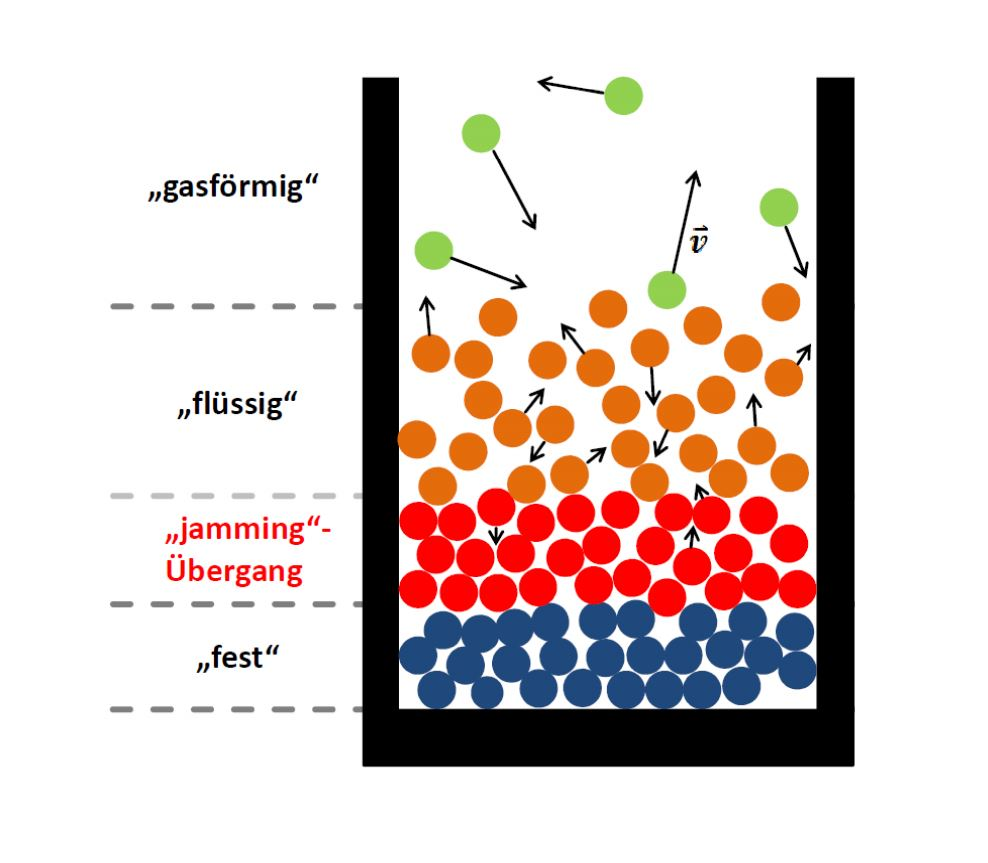
\includegraphics[scale=0.45]{Einleitung_1.jpg}
	\caption{Unterschiedliche Phasen eines Granulats  \cite{Darmstadt2015}}
\end{figure}	
\end{center}

Die in Abbildung 1.1 zu sehenden Phasen treten alle gleichzeitig während einer Anregung durch Vibration auf. \\
Im gasförmigen Zustand sind die Abstände der Partikel weit größer als der Partikeldurchmesser und die Partikel bewegen sich weitgehend unabhängig voneinander. \\
Der darunterliegende flüssige Zustand bietet bereits deutlich weniger Bewegungsfreiheit. Die mittlere freie Weglänge ist auf die Größenordnung der Partikel gesunken (fragen!). Man spricht auch von einem Glasübergang. \\
Charakteristisch für granulare Medien ist der \glqq jamming\grqq \ Übergang zwischen fest und flüssig. Hier ist keine Diffusion mehr möglich, die Partikel verbleiben also in ihrer Packungsposition und verklemmen mit ihrer Nachbarn. Bereits in diesem Zustand bilden sich sogenannte \glqq force chains\grqq \ heraus, über die die Kraftübertragung des Systems läuft. \\
Die \glqq force chains\grqq \ bilden sich im festen Zustand vollständig heraus und entstehen vor allem dadurch, das ein Teilchen deutlich mehr Nachbarn hat, als zu Stabilisation braucht. Da sich die Partikel amorph anordnen, verlaufen die \glqq force chains\grqq \ nicht homogen und isotrop, sondern willkürlich, was sich in einer unregelmäßigen Kraftverteilung ausdrückt. \cite{Darmstadt2015}, \cite{Fallturmexperiment}
Eine genaue Charakterisierung eines granularen Mediums ist mit der Methode von Castellanos (Zitieren) aus den XX Jahren möglich. Hierzu wird ein Wirbelbett genutzt, welches im folgenden Abschnitt erläutert wird.


\subsection{Wirbelbett}

Ganz allgemein ist ein Wirbelbett eine Konstruktion mit dessen Hilfe es möglich ist ein granulares Medium quantitativ zu vermessen. Ein sehr einfaches Wirbelbett kann man sich ungefähr so vorstellen:


\begin{figure}[h]
		\begin{center}

		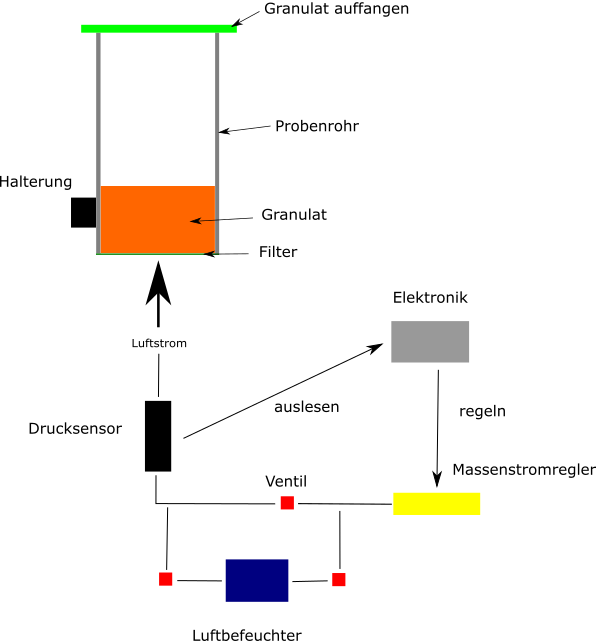
\includegraphics[scale=0.45]{Prinzip_Wirbelbett.png}
		\caption{Prinzip eines Wirbelbetts}
	\end{center}
\end{figure}	


Das im Probenrohr befindliche granulare Medium wird von unten mittels eines regelbaren Luftstrom durchströmt. Das Ziel ist hierbei den Zustand der sogenannten \glqq Fluidisation\grqq \ zu erreichen. Um diesen Zustand messtechnisch zu bestimmen, ist es nötig den über dem granularen Medium abfallenden Druck zu messen. Sobald dieser Druck konstant ist, ist der Zustand der Fluidisation erreicht. Der abfallende Druck wird hierbei über die Strömungsgeschwindigkeit des Luftstroms geregelt.


\section{Derzeitiger Stand und Probleme}


Das bisherige Wirbelbett besteht aus einem eingesteckten Röhrchen mit einem herkömmlichen Schwamm als Filter. Das Röhrchen und die Gaszufuhr sind beide auf einem hohlen Metallblock montiert und mittels Kleber wird der luftdichte Abschluss erreicht. \\
Das oben beschriebene Teil ist zur vertikalen Verstellbarkeit auf einen Geräteträger montiert, für die horizontale Verstellbarkeit sorgt eine Mikrometerschraube auf dem Geräteträger. 

\begin{figure}[h]
	\begin{center}
		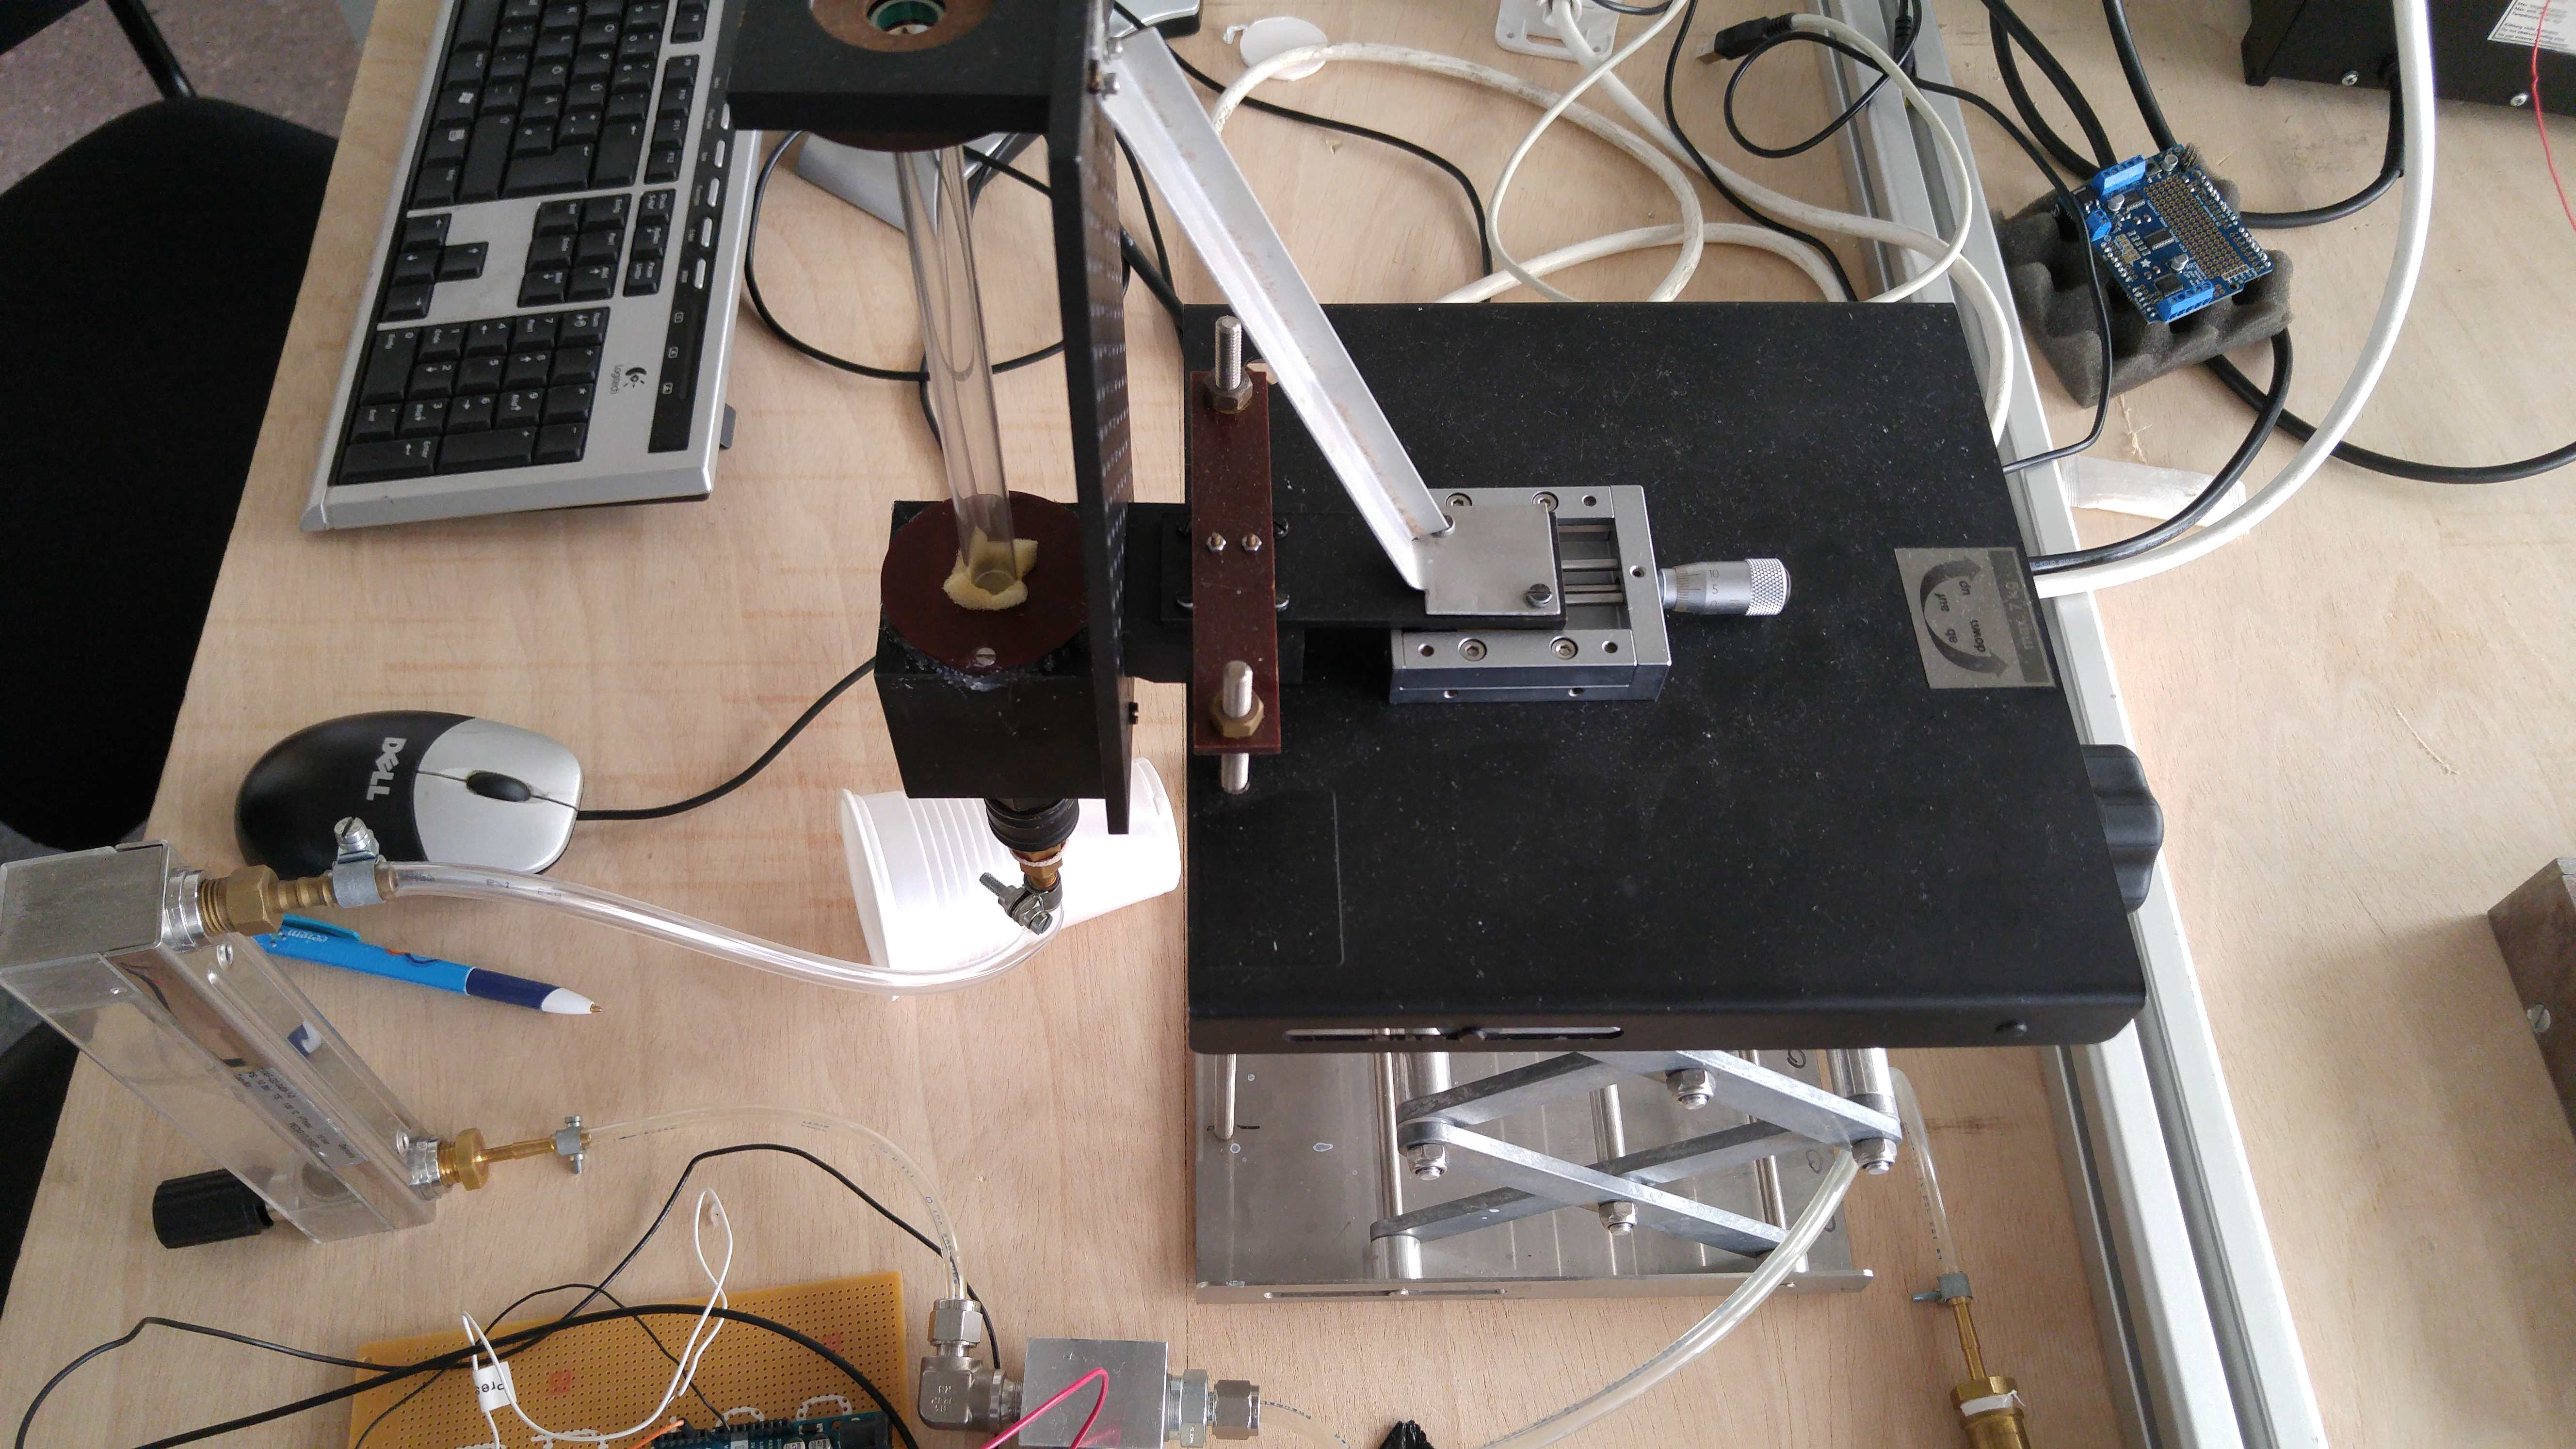
\includegraphics[scale=0.055]{Altes_Wirbelbett_oben.jpg}
		\caption{Wirbelbett}
	\end{center}
\end{figure}	


Die Gaszufuhr wird über flexible Plasikschläuche realisiert, die teils mit Klemmen und teils mit Muttern an den Geräteflanschen befestigt sind. \\
Die Elektronik zum Auslesen des Drucksensors liegt offen und anfällig auf dem Tisch, zudem kann der Druck noch nicht genau genug ausgelesen werden. Man bekommt ein Signal zwischen \SIrange{0}{10}{\volt} vom Sensor, das über einen Spannungsteiler auf \SIrange{0}{5}{\volt} reduziert wird. \\
Dieser Aufbau bringt eine Reihe von Problemen mit sich. Das größte Problem ist sicherlich, das nicht mit unterschiedlichen Probenrohrdurchmessern gemessen werden kann. Außerdem ist der luftdichte Anschluss am Probenrohr nicht gegeben, da dies nur mit dem Schwamm in eine Öffnung des Metallblocks gesteckt wird.
Weiterhin ist das Wirbelbett zwar vertikal und horizontal beweglich, aber der Geräteträger verhindert Messungen im Lichtstreuaufbau.
Die bisherige Verrohrung mit Plastikschläuchen ist nicht luftdicht und zu instabil um transportiert zu werden. \\


\begin{figure}[h]
	\begin{center}
		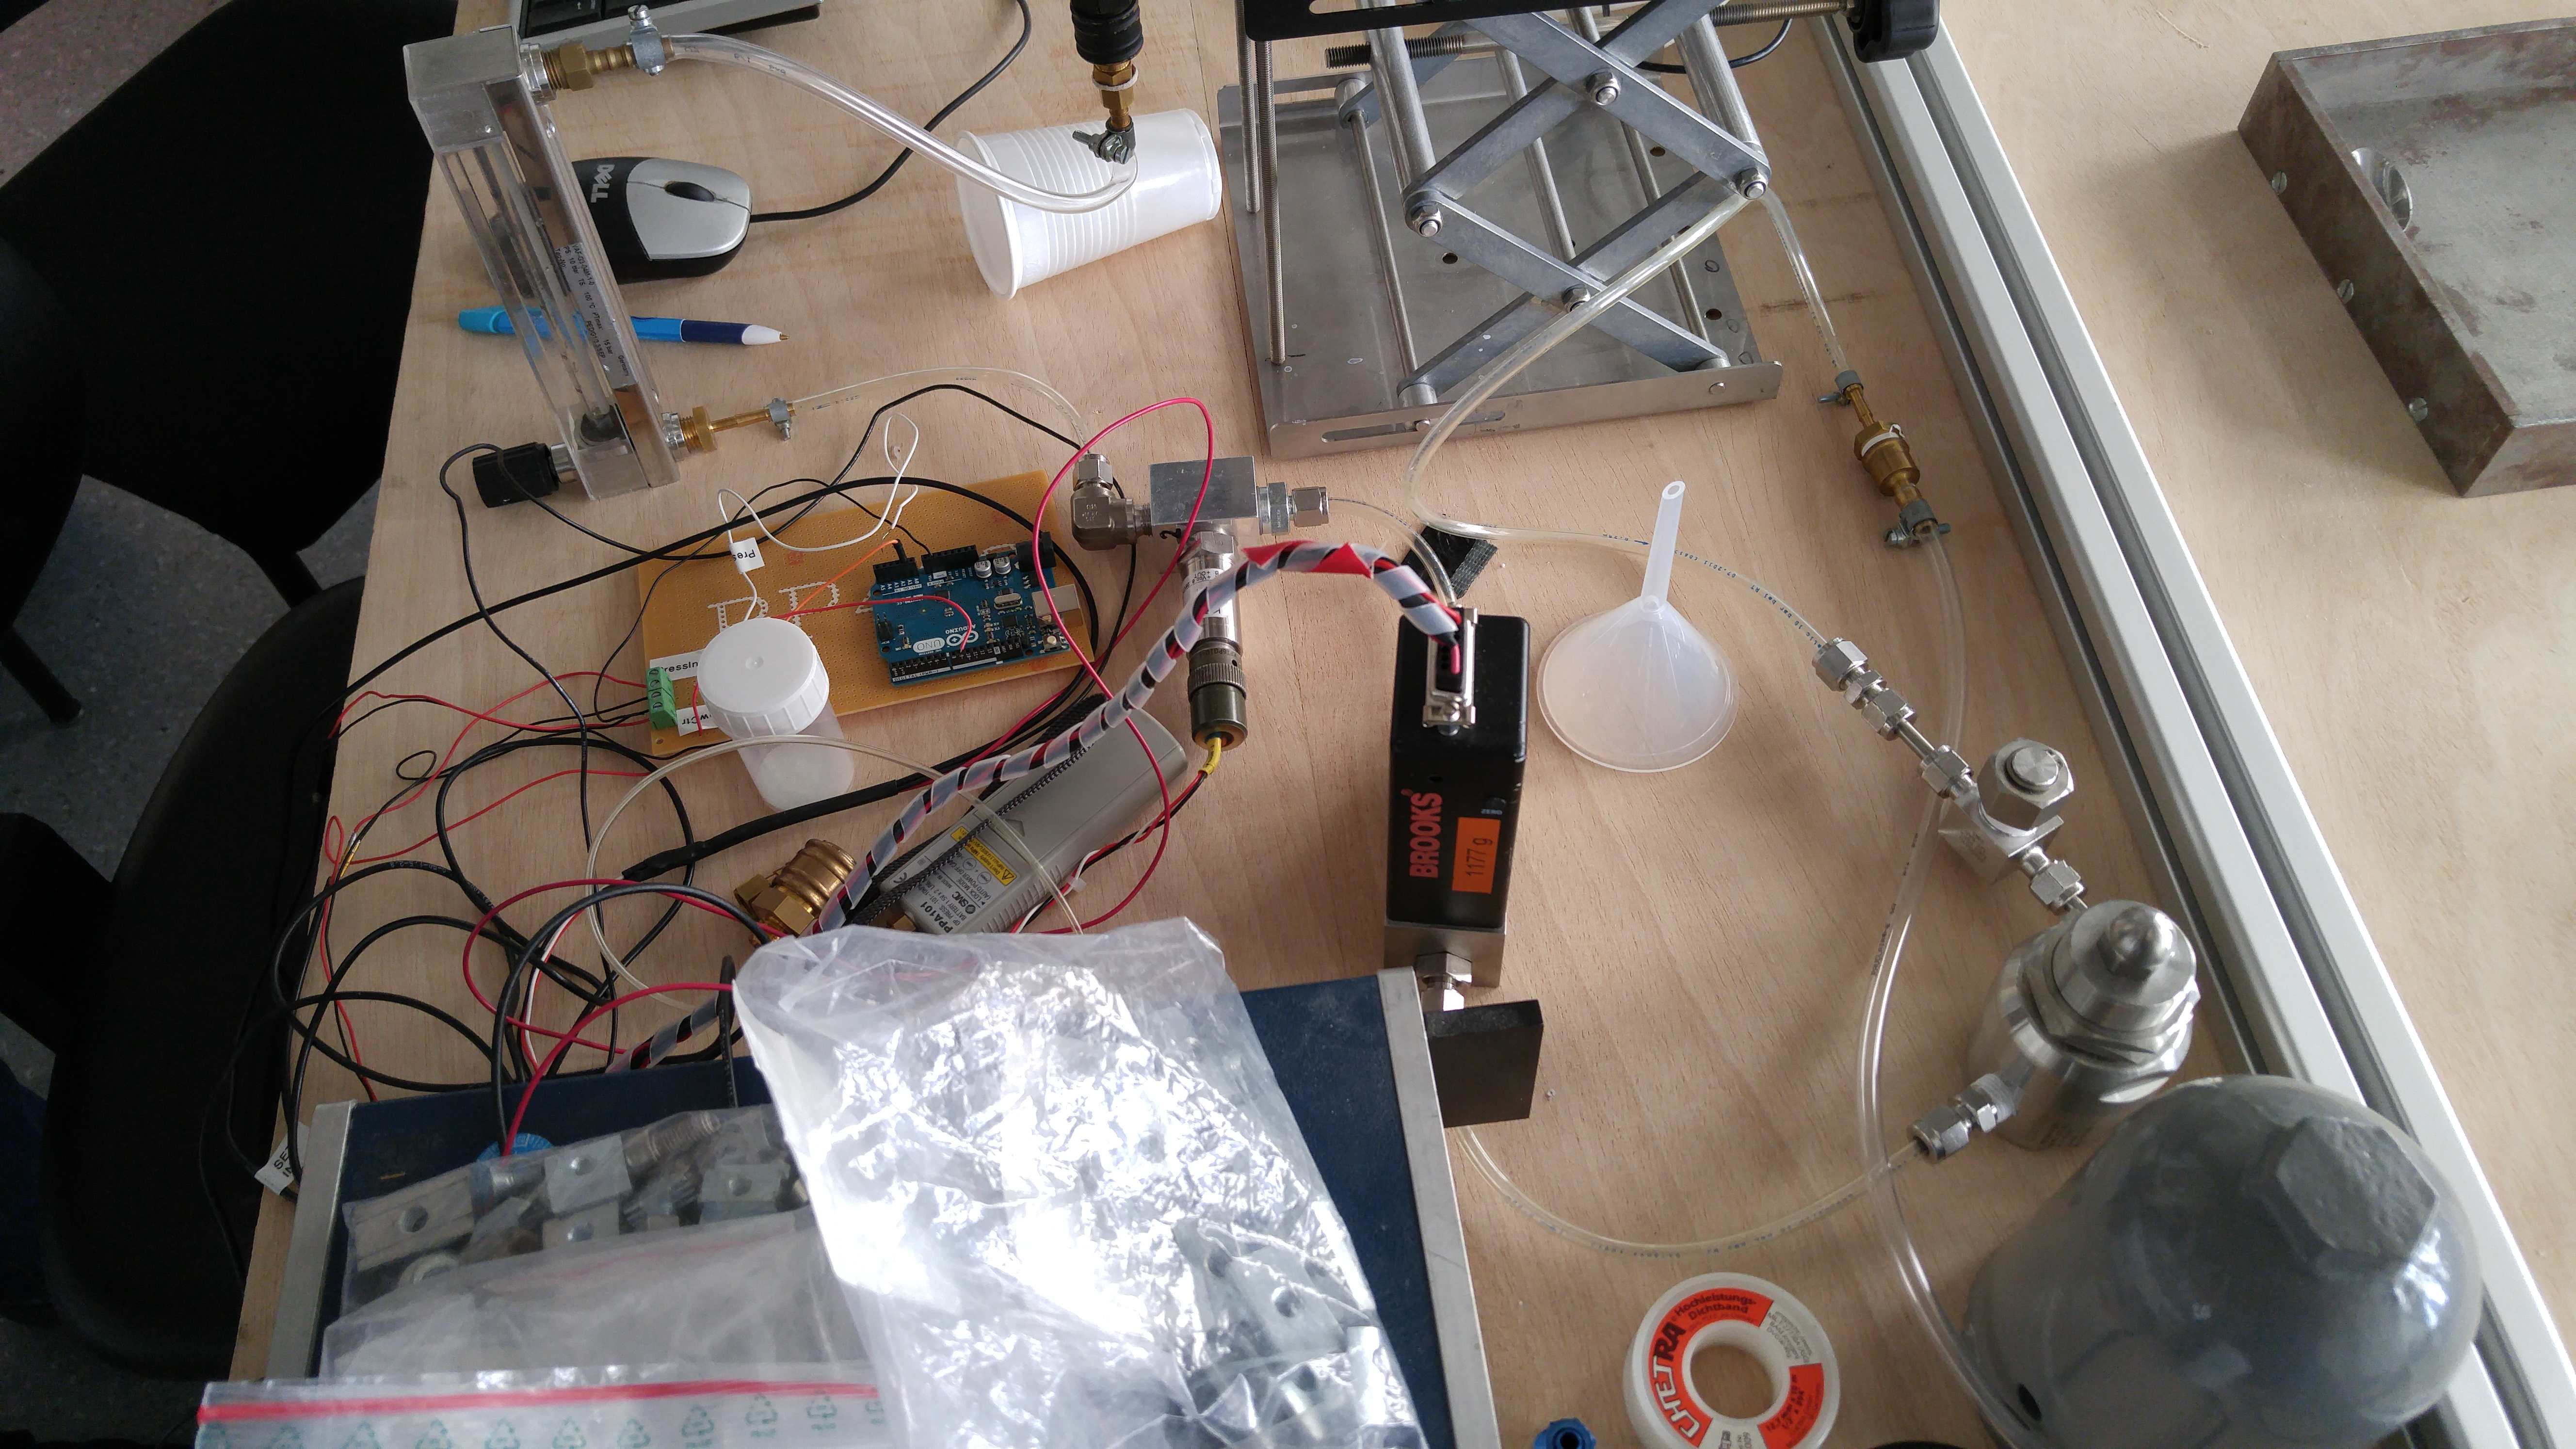
\includegraphics[scale=0.055]{Kabel_Rohrleitungen_alt.jpg}
		\caption{Verrohrung und Elektronik}
	\end{center}
\end{figure}


\section{Wissenschaftliche Fragestellung}

Wie schon Castellanos gezeigt hat, gibt es einen Zusammenhang zwischen dem Fluidisierungspunkt und der Teilchengröße des Granulats. Der hier gebaute Messaufbau soll das selbe Messprinzip nutzen wie schon Castellanos, also den Druckabfall in Abhängigkeit der Gasströmungsgeschwindigkeit. Beispielhaft sieht man in dem unten stehenden Diagramm ein Messprotokoll von Granulat mit xyz Eigenschaften.

\begin{figure}[h]
	\begin{center}
		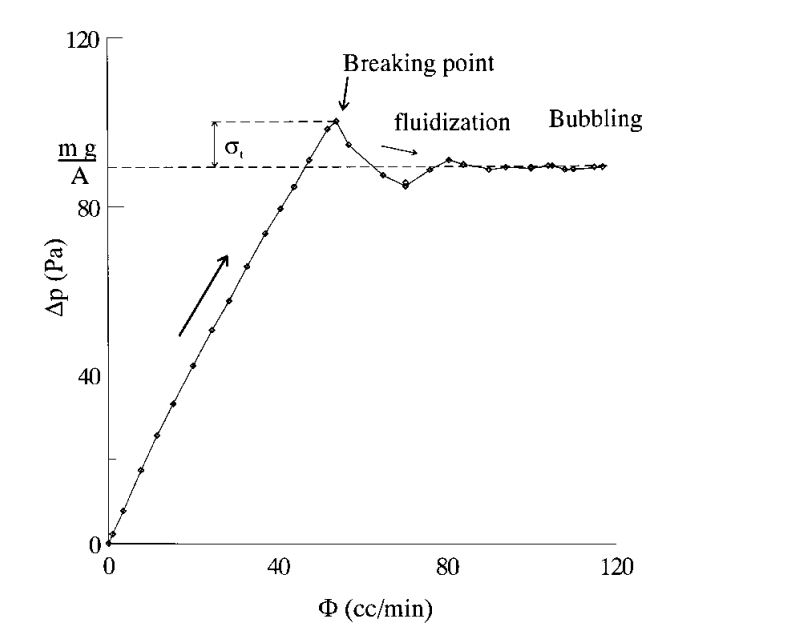
\includegraphics[scale=0.5]{Castellanos_Diagramm.jpg}
		\caption{\cite{Castellanos2000}}
	\end{center}
\end{figure}

Eine weiterführende Fragestellung ist nun, ob man den Fluidisierungspunkt kontrollieren kann, indem man die Partikel auf verschiedene Arten beschichtet oder anderweitig behandelt. Dazu muss eine große Bandbreite verschiedener Medien quantitaiv messbar sein. Die Realisierung eines solchen Messaufbaus ist Ziel dieser Arbeit. 


\section{Ziele der Arbeit}

In der Arbeit soll ein vorhandener Versuchsstand für quantitative Messungen neu gebaut werden, zudem soll der Versuchsstand sowohl mit Luft als auch mit Wasser betrieben werden können. Im ersten Teil werden die Probleme des bisherigen Setups analysiert und eine entsprechende Lösung für das Medium Luft konstruiert. \\ 
Der zweite Teil beschäftigt sich mit der Konzeption des Wasserbetriebs und dessen Umsetzung. \\
Konkrete Ziele des Praxisprojekts sind thematisch geordnet folgende:
Die Elektronik soll im Bezug auf das Auslesen des Drucksensors genauer gemacht und in ein Gehäuse verpackt werden. \\
Es soll ein neues Gassystem entworfen werden, das luftdicht und mechnanisch stabil ist. Weiterhin soll in das Gassystem ein Luftbefeuchter integriert werden. Zudem muss der Gasstrom regelbare Gasstrom auf Grund der größeren Probenröhrchendurchmesser erhöht werden.  \\
Das Wirbelbett soll insofern neugebaut werden, sodass mit verschiedenen dicken Probenröhrchen gemessen werden kann. Die Röhrchen sollen einfach und schnell wechselbar sein und auch das Probenmaterial muss einfach zu wechseln sein. Zur Unterbindung der Elektrostatik des granularen Mediums ist die Integration eines Luftionisators geplant. Weiterhin soll das Wirbelbett für eine korrekte Integration in den Lichtstreuaufbau horizontal und vertikal manipulierbar sein. \\
Zur Strukturierung der Arbeit wurden die einzelnen Ziele in folgende Arbeitspakete unterteilt:


\subsection{AP 1 - Analyse}

In den ersten zwei Wochen werden die Eckdaten den Projekts gesammelt und den Anforderungen zugeordnet. Zudem wird über die Materialwahl für das Wirbelbett entschieden und eine Stückliste aller Kaufteile für das Projekt insgesamt erstellt. Außerdem werden erste Lösungsansätze definiert, was wiederum in die Liste der Kaufteile einfließt.


\subsection{AP 2 - Elektronik}

In den Wochen zwei und drei soll das Gehäuse für die Elektronik gebaut werden und das Problem mit dem nicht genau genug auszulesenden Drucksensors gelöst werden. Dies soll zu Anfang geschehen, weil die Steuerelektronik für jegliche Steuerung zuständig ist und somit ohne diese das Wirbelbett nicht bedienbar ist. Zudem kann mit einem recht einfache Bauteil wie dem Gehäuse erste Erfahrungen mit dem 3D Drucker gesammelt werden.

\subsection{AP 3 - Gassystem}

Dieses Arbeitspaket umfasst auch zwei Wochen und beschäftigt sich mit dem Gassystem. Hier geht es insbesondere um das suchen und bestellen der geeigneten Teile für die Verrohrung und den Luftbefeuchter, sowie den Zusammenbau selbiger. \\
Der Entschluss dieses Arbeitspaket auch recht früh anzugehen, fiel da insbesondere Komponenten wie der Flowcontroller Lieferzeiten von sechs Wochen oder mehr haben. 

\subsection{AP 4 - Wirbelbett}

Die Wochen sechs bis acht sollen dazu genutzt werden das eigentliche Wirbelbett neu zu konstruieren. Um schnell und effektiv beurteilen zu können, ob die Ideen zielführend sind, soll ein 3D Drucker zur Prototypenerzeugung genutzt werden. Die finalen Teile sollen auch mit dem 3D Drucker hergestellt werden. \\
Dieser Abschnitt liegt direkt vor dem Testen, damit unmittelbar nach dessen Abschluss alle für den Testlauf nötigen Komponenten vorhanden sind.


\subsection{AP 5 - Tests}

In einem letzten Abschnitt sollen alle Komponenten im vollständigen Aufbau getestet werden. Hier soll evaluiert werden, ob alle Anforderungen erfüllt wurden und ob es noch Mängel gibt. Kleinere Mängel sollen noch in dieser Phase behoben werden, während bei größeren analysiert werden muss wie damit umzugehen ist. Wenn möglich werden auch Messkurven des alten Messaufbaus und des neuen verglichen und diskutiert.





















